%\subsection{Tier0}

%IPv6 readiness of Tier-1 sites
 
%Since the very beginning of the LHC project the transport protocol IPv4 was connecting the world wide distributed sites. Since most LHC collaborating sites have a long history and in the beginning of the IPv4 address distribution applied for substantial address space they are not facing any IPv4 shortage at their institution However, after long and intense discussions eventually a
The approved timeline for IPv6 readiness of the Tier-1 sites was defined to be April 2018, but not all succeeded.
%After that date IPv6 only sites should be able to exchange data with the storage systems of the LHC tier-1 sites.  
%The matching of this timeline was quite different. 
Some Tier-1 sites like PIC in Spain or the distributed nordic NDGF Tier-1 were IPv6-ready long before the deadline. Some of the other sites reached the goal on time while others are still not fully IPv6-ready. 
%The IPv6 readiness of a site can be split into LHCOPN, LHCONE, General Purpose Internet (GPI), PerfSONAR Monitoring and the productions IPv6 readiness of a site. The following table shows the first three items of the list of each LHC tier-1:

%Figure \ref{LHCOPN+ONE_status.png} (LHCOPN/ONE IPv6 deployment)

 
%For LHC three major file transfer server (FTS) are organizing the file storage exchange of the experiments. Of this FTS servers at CERN, FNAL and BNL only the one at CERN is a dual-stack, the others are still only running on IPv4. BNL had a dual-stack up for some time, but due to problems with the file transfers switched back to IPv4 and changed the configuration to prefer IPv4 over IPv6. These transfer problems occurred only between IPv4 only sites.
%Using IPv6 is more than being connected by a newer and better protocol with a much larger address space. Introducing IPv6 within the sites requested programs to be analysed and checked for their IPv6 readiness. If they were not, it was and is neceessary to find alternatives. 

Some Tier-1 sites encountered technical problems with their transition.
%were confronted with difficult obstacles. 
For example at DE-KIT the IPv6 deployment was designed as a dual-homed architecture
%in the first approach deployed. 
and began with the IPv6 deployment for 
%the LHC VO 
CMS only. The motivation for dual-homing resulted from their current IPv4 deployment,
%since it is based on two IPv4 addresses, 
of one internal private address, and 
%a smaller number on 
hosts/servers with a second public address applied to a different (virtual) interface. 
%The private and public addresses are attached to different routing engines each with a routing policy designed specifically for the requirements. The private addresses are directed straight to the firewall for external communication, whereas the public addresses are able to reach all trusted sites via LHCOPN and LHCONE via a firewall-bypass. 
Since all hosts should receive only one IPv6 address, the first approach was to assign the IPv6 address to the so-called "internal" interface with the private address. 
%After deploying, it was discovered that 
In this scenario, a large number of transfers were failing. 
%After analyzing this issue it was found out that the so-called 
Analysis showed that the dCache-Doors require a dual-stack deployment instead of dual-homed. A dual-stack configuration was tested but transfers were still failing. After discussion with the dCache developers and problems also identified in gridftp, KIT decided to implement a dual-stack only environment.
%Since this was effecting only two CMS dCache-Door servers, a workaround was implemented which offered a dual-stack deployment. In theory with dual-stack dCache-Doors and dual-homed dCache-Pools IPv6 was realised, however, it failed. Under certain circumstances transfers did just not work out. The FTS at CERN was initiating transfers and communicating with KIT’s  dCache via IPv6. If those file transfers took place between IPv4 only sites, dcache had to change protocol from IPv6 to IPv4 and in other cases the actual transfer was  executed by gridftp, yet the transfer failed. Confronted with all these issues, at DE-KIT the decision was made to redesign the deployment to a dual-stack only environment.  Communication and discussions with dcache developers followed. They pointed to one issue at the protocol stack of gridftp, which had not been implemented rfc conform. But later it was discovered that changing some lines of code in dcache could have solved the issue.
  
In the beginning of 2018, EOS at CERN was upgraded to a version that supported IPv6.  
As soon as the EOS instances of the LHCb and ALICE experiments got a AAAA DNS records for their public nodes, an important increase of IPv6 traffic was noticed on the CERN central firewall, moving from few hundreds of Mbps to almost 10Gbps. 
Figure \ref{tier0-traffic.png} shows the traffic increase when the EOS dual-stack version was introduced.
 
This increased traffic began to saturate CERN's IPv6 firewall, so in June 2018 a
%increase posed some worries, because the IPv6 firewall path was limited to 10Gbps and was actually saturating now and then. So in June 2018 it was implemented the HTAR (High Throughput Alternative Route) 
firewall bypass was deployed for IPv6,
% action that has allowed 
thereby allowing the activation of dual stack access also for the ATLAS and CMS EOS instances.    
 
%The HTAR firewall bypass is a framework that allows some well known, high volume traffic to bypass the statefull inspection of the CERN central firewall. This framework has been in place for many years for IPv4, but the IPv6 part was not implemented initially because of limitation on the network hardware and lately because of a lack of IPv6 traffic.  

Even with all these unexpected obstacles the LHC Tier-1 centers are close to being fully IPv6 dual-stack. The only sites not yet complete are FNAL, BNL, KIT and one of the Russian Sites, namely RRC-KI-T1. 
%Since Triumf got dual-stack ready last month all other sites ready yet. Looking a little closer to the still pending sites: 
BNL is dual-stack ready, but they currently prefer IPv4 over IPv6; KIT's deployment from dual-homed to dual-stack is now deployed for Belle2 and CMS and the remaining VOs will follow soon; 
FNAL will enable their IPv6 dual-stack setup at the beginning of 2019; the Russian site is also preparing its IPv6 environment.

%All LHC tier-1 sites will get, even when some sites did not match the timeline, soon IPv6 ready and with the enabled HTAR at CERN and similar deployments at other LHC tier-1 centres ready for high IPv6 data throughput.

%\begin{figure}[h!]
%\centering
%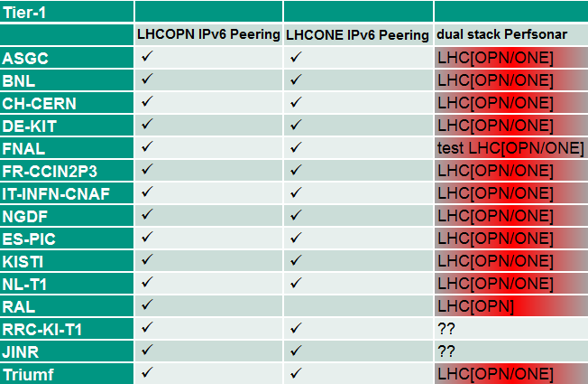
\includegraphics[width=5.6 in]{LHCOPN+ONE_status.png}
%\caption{LHC Tier-1 sites LHCOPN and LHCONE and PerfSONAR readyness status}
%\label{fig:LHC[OPN/ONE] Tier-1 readyness status}
%\end{figure}

\begin{figure}[h!]
\centering
%\includegraphics[width=5.6 in]{tier0-ipv6-firewall-traffic.png}
\includegraphics[width=13cm]{tier0-ipv6-firewall-traffic.png}
\caption{IPv6 traffic through the CERN central firewall, period Sept 2018-Sept 2019}
\label{fig:tier0-traffic}
\end{figure}
